\documentclass[]{../template/Report}
\settemplatedir{../template/} %设置模板文件夹路径
\exname{万用表的设计} %实验名称
\instructor{} %指导教师
\class{} %班级
\extable{}
\name{} %姓名
\stuid{} %学号

\nyear{2025} %年
\nmonth{9} %月
\nday{24} %日
\nweekday{三} %星期几
\daypart{上} %上午/下午
\redate{} %如有实验补做,补做日期
\resitu{} %情况说明:
\begin{document}
\makecover

\section{预习报告}
\subsection{实验综述}
\subsubsection{测量电流计的内阻}
    利用替代法或中值法测量电流计内阻。这里使用替代法(\cref{tidaifa}),先将电流计与标准电流表同时串接在回路中。调节可变电阻使回路电流为合适大小$I_0$,再将电流计用电阻箱换下,调整电阻箱阻值,使回路电流仍为$I_0$,此时电阻箱的阻值即为电流计的内阻。
    \begin{figure}[htbp]
        \centering
        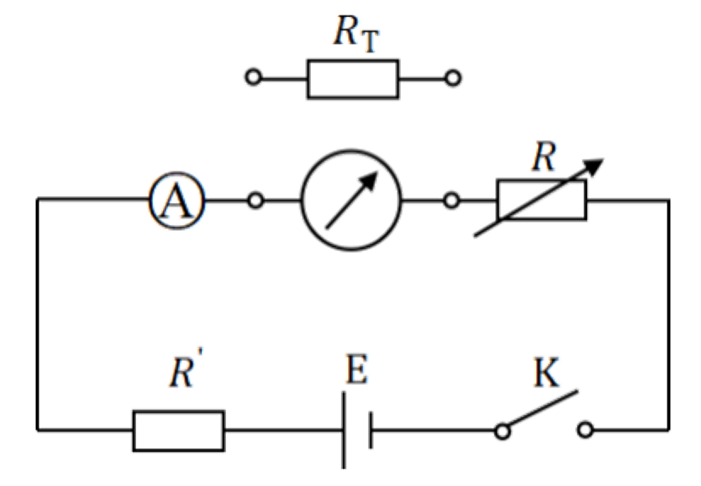
\includegraphics[width=0.4\textwidth]{tidaifa.png}
        \caption{替代法测量电流计内阻}
        \label{tidaifa}
    \end{figure}

\subsubsection{设计、改装并校准多量程电流表}
    设计多量程电流表电路如\cref{duoliangchengdianliu}所示。由并联电压相等,分别列出接量程$I_1(\SI{10}{mA})$、量程$I_2(\SI{5}{mA})$时的方程:
    \begin{equation}
        \begin{cases}
            (R_g+R_2)I_g = R_1 (I_1 - I_g)\\
            (R_1+R_2)(I_2 - I_g) = R_g I_g
        \end{cases}
    \end{equation}
    计算出$R_1 = \frac{R_gI_gI_2}{I_1(I_2-I_g)}$、$R_2 = \frac{R_gI_g(I_1-I_2)}{I_1(I_2-I_g)}$,将电阻箱调为对应阻值接入电路,即得多量程电流表。

    然后,用\cref{duoAjiaoyan}所示电路校验多量程电流表,记录数据并分析误差。最后校准多量程电流表,若测量值偏小,则增大电阻箱内阻,反之则减小电阻箱内阻,直至测量值与标准电流表读数相符。
    \begin{figure}[htbp]
        \centering
        \begin{subfigure}[b]{0.45\textwidth}
            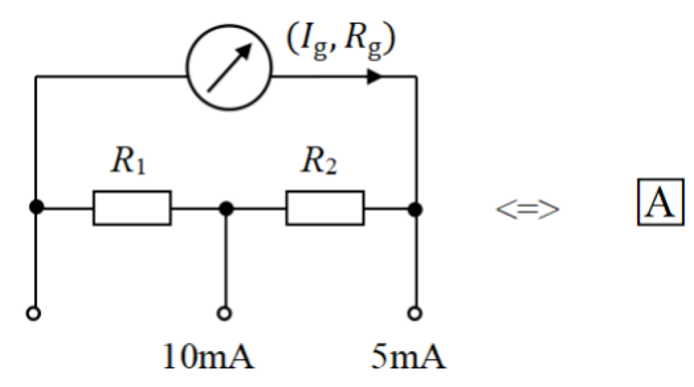
\includegraphics[width=\textwidth]{duoliangchengdianliu.png}
            \caption{多量程电流表设计电路}
            \label{duoliangchengdianliu}
        \end{subfigure}
        \hfill
        \begin{subfigure}[b]{0.45\textwidth}
            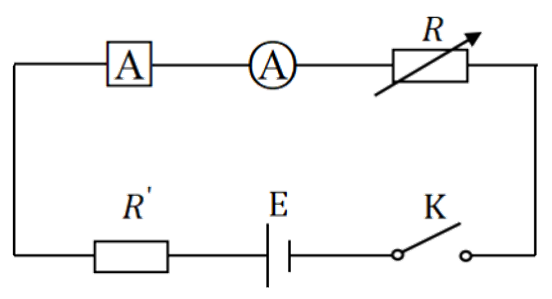
\includegraphics[width=\textwidth]{duoAjiaoyan.png}
            \caption{多量程电流表校验电路}
            \label{duoAjiaoyan}
        \end{subfigure}
    \caption{多量程电流表相关电路}
    \end{figure}

\subsubsection{设计、改装并校准多量程电压表}
    设计多量程电压表电路如\cref{duoliangchengdianya}所示。由串联电流相等,分别列出接量程$U_1(\SI{5}{V})$、量程$U_2(\SI{10}{V})$时的方程:
    \begin{equation}
        \begin{cases}
            (R_g'+R_3)I_g' = U_1\\
            (R_g'+R_3+R_4)I_g' = U_2\\
            R_g' = \frac{R_g(R_1+R_2)}{R_g+R_1+R_2}
        \end{cases}
    \end{equation}
    计算出$R_3=\frac{U_1}{I_g'}-R_g'$、$R_4 = \frac{U_2-U_1}{I_g'}$,将电阻箱调为对应阻值接入电路,即得多量程电压表。

    然后,用\cref{duoVjiaoyan}所示电路校验多量程电压表,记录数据并分析误差。最后校准多量程电压表,若测量值偏小,则增大电阻箱内阻,反之则减小电阻箱内阻,直至测量值与标准电压表读数相符。
    \begin{figure}[htbp]
        \centering
        \begin{subfigure}[b]{0.45\textwidth}
            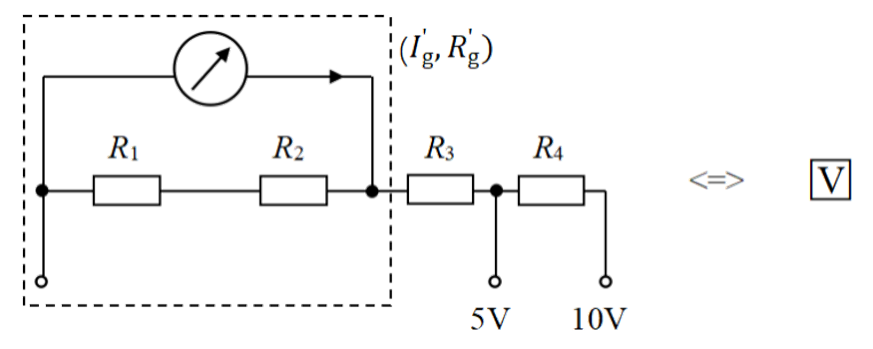
\includegraphics[width=\textwidth]{duoliangchengdianya.png}
            \caption{多量程电压表设计电路}
            \label{duoliangchengdianya}
        \end{subfigure}
        \hfill
        \begin{subfigure}[b]{0.45\textwidth}
            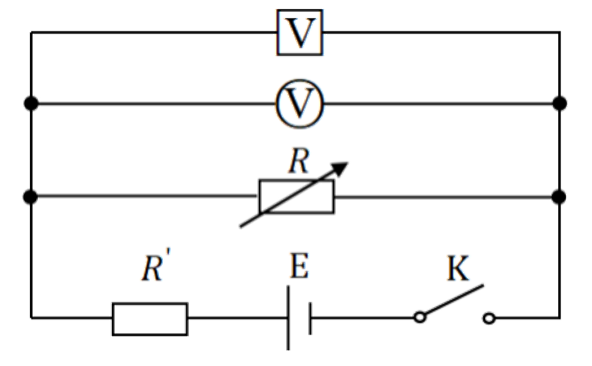
\includegraphics[width=\textwidth]{duoVjiaoyan.png}
            \caption{多量程电压表校验电路}
            \label{duoVjiaoyan}
        \end{subfigure}
        \caption{多量程电压表相关电路}
    \end{figure}

\subsubsection{改装欧姆表}
    设计欧姆表电路如\cref{ohm}所示。首先短接$a,b$,调节$R_6$使电流计满偏,此时有$I_o = I_g' = \frac{\epsilon}{R_g'+R'}$,其中$R'$为回路中其他所有电阻之和。当不同$R_x$接入回路时,有$I_x = \frac{\epsilon}{R_g'+R'+R_x}$,记录$I_x$和$R_x$的值,并可在电流计面板上刻上刻度以显示不同阻值。特别地,当$I_x=\frac{I_o}{2}$时,有$R_x = R_g' + R'$称为欧姆表的中值电阻。
    \begin{figure}[htbp]
        \centering
        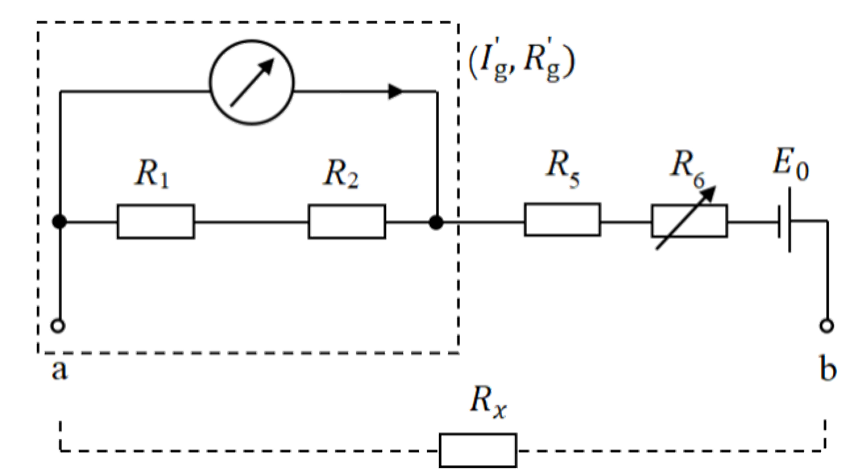
\includegraphics[width=0.4\textwidth]{ohm.png}
        \caption{欧姆表设计电路}
        \label{ohm}
    \end{figure}
\subsection{实验重点}
\begin{enumerate}
    \item 掌握电流计的工作原理及其内阻的测量方法;
    \item 学会多量程电流表和电压表的设计、改装与校准方法;
    \item 理解欧姆表的工作原理及其改装方法。
\end{enumerate}
\subsection{实验难点}
\begin{enumerate}
    \item 设计多量程电流表和电压表时,计算并调节电阻箱阻值以实现所需量程;
    \item 理解并应用误差分析方法,确保实验结果的准确性和可靠性;
    \item 正确应用电路连接和调试技巧,确保实验过程顺利进行;
    \item 正确进行实验设计和数据分析。
\end{enumerate}
\begin{fullreportonly}
    \section{原始数据(20分)}
(将有老师签名的“自备数据记录草稿纸”的扫描或手机拍摄图粘贴在下方,完整保留姓名,学号,教师签字和日期。)

\section{结果与分析(60分)}
\subsection{数据处理与结果(30分)}
(列出数据表格、选择适合的数据处理方法、写出测量或计算结果。)

\subsection{误差分析(20分)}
(运用测量误差、相对误差或不确定度等分析实验结果,写出完整的结果表达式,并分析误差原因。)

\subsection{实验探讨(10分)}
(对实验内容、现象和过程的小结,不超过100字。)

\section{思考题(10分)}
(解答教材或讲义或老师布置的思考题,请先写题干,再作答。)
\end{fullreportonly}
\insertnotes
\end{document}
